\documentclass[twocolumn,10pt]{article}
\usepackage[margin=1.8cm]{geometry}
\usepackage{amsmath,amssymb}
\usepackage{graphicx}
\usepackage{booktabs}
\usepackage{caption}
\usepackage[colorlinks=true,linkcolor=blue,citecolor=blue,urlcolor=blue]{hyperref}

\captionsetup{font=small,labelfont=bf}
\setlength{\parskip}{2pt}
\graphicspath{{../figures/}}

\newcommand{\bd}{\hat b^\dagger}
\newcommand{\avg}[1]{\langle #1 \rangle}

\title{\vspace{-1.5em}\textbf{Emergence of Statistical-Ensemble Equivalence in a\\
Two-Dimensional Interacting Quantum Lattice Gas}}
\author{Prasang Das \and Aryan Shakya \and Dhruv Thakur}
\date{\small A computational statistical-mechanics study by exact diagonalization}

\begin{document}
\twocolumn[
\maketitle
\begin{center}
\begin{minipage}{0.92\textwidth}
\small\textbf{Abstract.}
We study the equivalence of the microcanonical, canonical, and grand-canonical
ensembles in a two-dimensional hard-core Bose--Hubbard model---an interacting
\emph{quantum lattice gas}---as a controlled function of system size and
interaction strength. Using full-spectrum exact diagonalization on square
lattices of $L\times L=4,9,16$ sites, in every conserved particle-number sector,
we compute each ensemble's thermodynamics from a single shared set of
eigenvalues. We find that finite-difference microcanonical temperature and
chemical potential are numerically ill-conditioned on the small bounded discrete
spectra reachable by exact diagonalization, and we therefore quantify ensemble
equivalence through well-conditioned fluctuation observables: the relative energy
fluctuation $\sigma_E/|\avg{E}|$ (microcanonical$\leftrightarrow$canonical) and
the relative number fluctuation $\sigma_N/\avg{N}$
(canonical$\leftrightarrow$grand-canonical), together with the per-site
canonical--grand energy gap. For the non-interacting ($V=0$) and repulsive
($V/t=+2$) gases, all three discrepancy metrics decrease monotonically with
system size, following approximate power laws in $M=L^2$ and demonstrating the
expected emergence of equivalence. For the attractive gas ($V/t=-2$), the
relative number fluctuation remains large and essentially size-independent
($\sim M^{-0.12}$), signalling the breakdown of canonical--grand equivalence
associated with the clustering/phase-separation instability of an attractive
lattice gas.
\vspace{1em}
\end{minipage}
\end{center}
]

\section{Introduction}
The equivalence of statistical ensembles is a foundational assertion of
equilibrium statistical mechanics: in the thermodynamic limit, the
microcanonical ($N,V,E$), canonical ($N,V,T$), and grand-canonical ($\mu,V,T$)
descriptions yield the same intensive thermodynamics. It is a \emph{limit}
statement. For finite systems---nanoscale devices, cold-atom quantum simulators,
and all numerically exact many-body calculations---the ensembles differ by
corrections that vanish only as the particle number grows. Understanding the rate
and mechanism of this convergence, and when it fails, is both conceptually
central and practically important.

We address the question in a minimal but nontrivial quantum model and ask: how
does the equivalence of the three ensembles emerge in an interacting quantum
lattice gas as system size increases, and how do quantum hopping and interaction
affect the finite-size discrepancies? We study the two-dimensional hard-core
Bose--Hubbard model---a quantum lattice gas in the statistical-mechanical sense
(indistinguishable quantum particles on lattice sites with tunnelling and
interaction), realized by ultracold bosons in optical lattices in the hard-core
limit. This is unrelated to the identically named ``quantum lattice-gas
automaton'' of quantum computing; we study the many-body physical model.

Our methodology is correctness-first: we build the Hamiltonian in each conserved
$N$-sector, validate against independent analytic and brute-force results,
diagonalize fully, and only then compare ensembles. A central methodological
finding---that finite-difference microcanonical $T$ and $\mu$ are unreliable at
these sizes---leads us to anchor the study on fluctuation observables that are
smooth sums over the spectrum.

\section{Model and methods}
\subsection{Hamiltonian}
On an $L\times L$ square lattice with $M=L^2$ sites we consider hard-core bosons
with nearest-neighbor hopping and interaction,
\begin{equation}
\hat H=-t\!\sum_{\langle i,j\rangle}\!\big(\bd_i \hat b_j+\bd_j \hat b_i\big)
+V\!\sum_{\langle i,j\rangle}\!\hat n_i \hat n_j,\quad \hat n_i=\bd_i\hat b_i,
\end{equation}
with the hard-core constraint $\hat n_i\in\{0,1\}$,
$\hat b_i^2=(\bd_i)^2=0$. Here $t$ is the hopping amplitude, $V$ the
nearest-neighbor interaction ($V>0$ repulsive, $V<0$ attractive). We set $k_B=1$
and measure energy in units of $t$, so the controls are $V/t$, $T/t$, $\mu/t$,
and use periodic boundary conditions. The Hamiltonian conserves particle number,
$[\hat H,\hat N]=0$, hence is block-diagonal in $N$: we diagonalize each
fixed-$N$ block and reuse the eigenvalues in all three ensembles. In the
occupation basis hard-core bosons carry no inter-site exchange sign, so each
hopping element is $-t$ and every block is real symmetric.

\subsection{Basis and exact diagonalization}
A basis state is an occupation string encoded as an integer whose $i$-th bit is
$n_i$. The full space has dimension $2^M$; the fixed-$N$ sector has dimension
$\binom{M}{N}$. Because the canonical and grand partition functions sum over the
\emph{entire} spectrum, we require all eigenvalues of each block and use a dense
symmetric eigensolver (\texttt{eigvalsh}) rather than an iterative method. The
ceiling is the half-filling sector $\binom{M}{M/2}$; for $L=4$ this is $12\,870$,
diagonalized in minutes. Per-sector spectra are cached once and reused.

\subsection{Three ensembles from one spectrum}
With $E_{N,\alpha}$ the $\alpha$-th eigenvalue of sector $N$:
microcanonical $\Omega(E,N;\Delta E)=\#\{\alpha:E\le E_{N,\alpha}<E+\Delta E\}$,
$S=\ln\Omega$; canonical $Z_N=\sum_\alpha e^{-\beta E_{N,\alpha}}$,
$\avg{E}_N=-\partial_\beta\ln Z_N$, $C_V=\beta^2\mathrm{Var}(E)$;
grand-canonical $\Xi=\sum_N e^{\beta\mu N}Z_N$,
$\avg{N}=\sum_{N,\alpha}N p_{N,\alpha}$,
$\partial_\mu\avg{N}=\beta\mathrm{Var}(N)$, with
$p_{N,\alpha}=e^{-\beta(E_{N,\alpha}-\mu N)}/\Xi$. All partition functions use a
log-sum-exp shift to prevent overflow.

\subsection{Measuring equivalence: fluctuation metrics}
Extracting $T,\mu$ from microcanonical finite differences is fragile on small
bounded discrete spectra: $S(E)=\ln\Omega$ is a jagged window-dependent
histogram whose derivative diverges in spectral gaps (low $T$) and flips sign
near the density-of-states maximum (the negative-temperature region of a bounded
spectrum). We verified this across surface-entropy, Gaussian-broadened, and
Gibbs/volume-entropy variants; it is an intrinsic small-system limitation.

We therefore quantify equivalence through smooth spectral sums requiring no
differentiation:
\begin{align}
r_E&\equiv\frac{\sigma_E}{|\avg{E}|}=\frac{\sqrt{\mathrm{Var}(E)}}{|\avg{E}|}\sim M^{-1/2},\\
r_N&\equiv\frac{\sigma_N}{\avg{N}}=\frac{\sqrt{\mathrm{Var}(N)}}{\avg{N}}\sim M^{-1/2},\\
\Delta_E/M&\equiv\frac{1}{M}\big|\avg{E}_{\text{grand}}-\avg{E}_{\text{can}}\big|.
\end{align}
$r_E$ measures the sharpness of the canonical energy saddle (micro$\leftrightarrow$canonical);
$r_N$ measures the number-distribution width at $\mu^{*}$ tuned so $\avg{N}=N$
(canonical$\leftrightarrow$grand). Since $\avg{N}(\mu)$ is monotone
($\partial_\mu\avg{N}=\beta\mathrm{Var}(N)>0$), $\mu^{*}$ is unique and found by
Brent's method to $10^{-10}$. Finite-difference $T,\mu$ are kept only as a
noisy secondary diagnostic.

\section{Validation}
The implementation was validated against independent references, all encoded as
automated tests: (i) Hermiticity of every block to machine precision; (ii)
sector dimension $\binom{M}{N}$ with sectors partitioning $2^M$; (iii)
particle-number conservation---an independently built full-space Hamiltonian is
block-diagonal in $N$ and its spectrum equals the union of per-sector spectra to
$10^{-10}$; (iv) the analytic $V=0$, $2\times2$, $N=1$ spectrum
$\{-2t,0,0,+2t\}$ (four-site ring); (v) the trace identity $\mathrm{Tr}\,H=V\sum
(\text{occupied bonds})$; (vi) the $T\to0$ and $T\to\infty$ limits of $\avg{E}$,
$S$, and $C_V$. Ground-state energies ($V=0$): $E_0/t=-2.828,-10.347,-18.000$ for
$L=2,3,4$. The full suite (57 tests) passes.

\section{Results}
\subsection{Spectrum and density of states}
Figure~\ref{fig:dos} shows the per-sector spectrum and total density of states
for the $L=4$ free gas. The bounded spectrum with a central DOS maximum is the
structural origin of the negative-temperature region and of the
finite-difference thermometry failure.
\begin{figure}[t]\centering
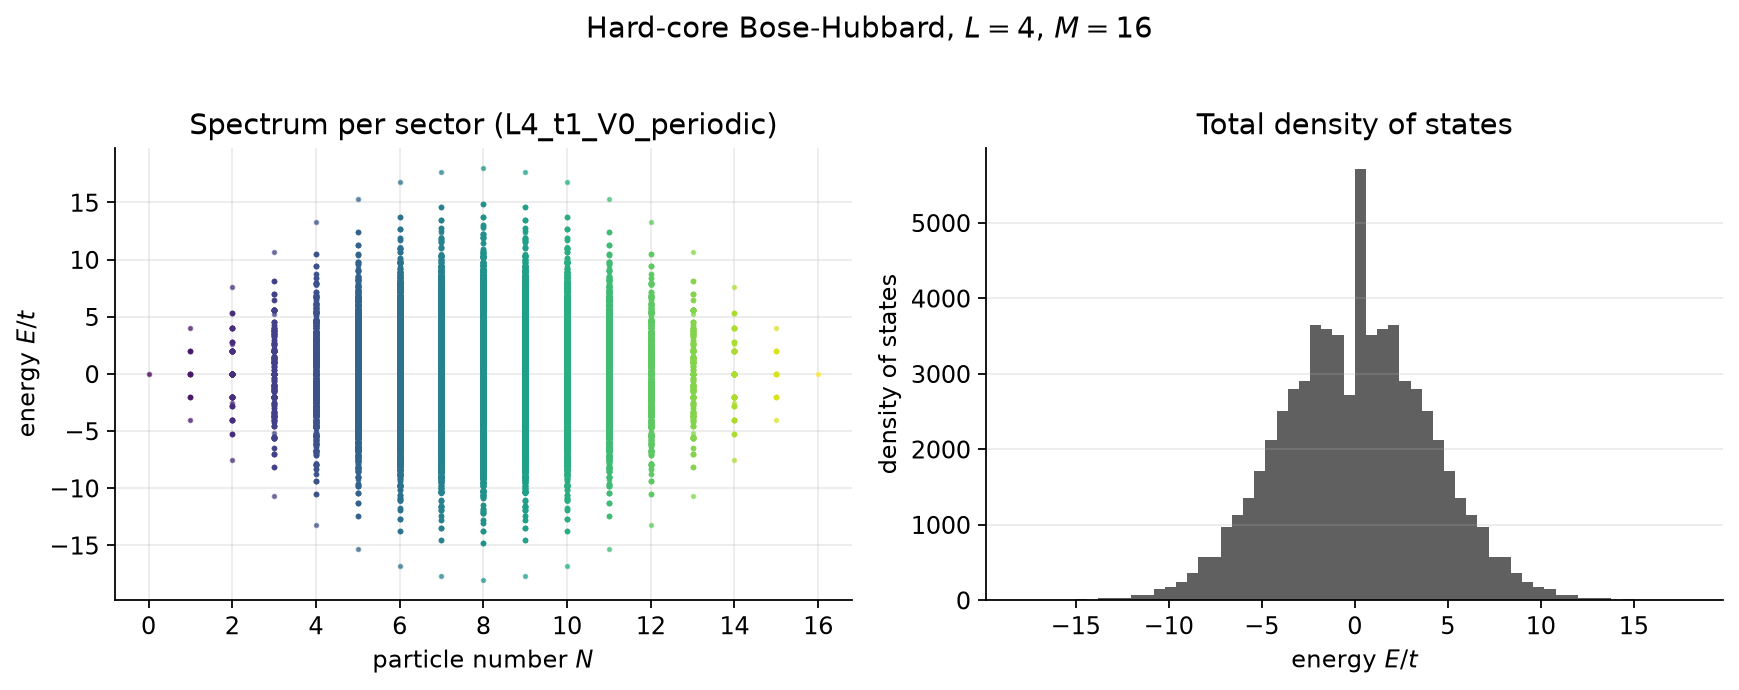
\includegraphics[width=\columnwidth]{fig1_spectrum_dos.png}
\caption{Eigenvalues per sector (left) and total density of states (right),
$L=4$, $V=0$.}\label{fig:dos}
\end{figure}

\subsection{Heat capacity}
The canonical heat capacity (Fig.~\ref{fig:cv}) shows a single broad
Schottky-like peak, vanishing as $T\to0$ and $T\to\infty$. Repulsion shifts the
peak to higher $T$, attraction to lower $T$, preserving the Schottky form.
\begin{figure}[t]\centering
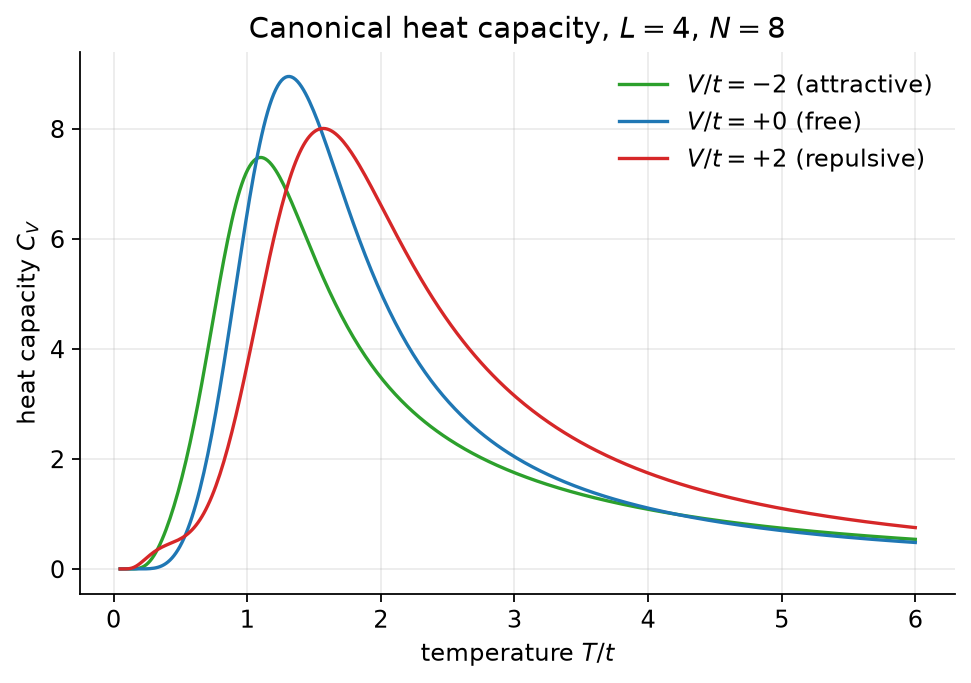
\includegraphics[width=\columnwidth]{fig2_heat_capacity.png}
\caption{Canonical $C_V(T)$ at half filling ($L=4$, $N=8$) for free, repulsive,
and attractive gases.}\label{fig:cv}
\end{figure}

\subsection{Grand-canonical filling and fluctuations}
Figure~\ref{fig:fill} shows filling versus $\mu$ at $\beta t=1$; all curves cross
half filling at $\mu=0$ (particle--hole symmetry), with $L=3,4$ converging toward
a common thermodynamic profile while $L=2$ deviates. Figure~\ref{fig:varn} shows
$\mathrm{Var}(N)$ and the compressibility $\kappa\sim\mathrm{Var}(N)/\avg{N}^2$,
peaking near half filling.
\begin{figure}[t]\centering
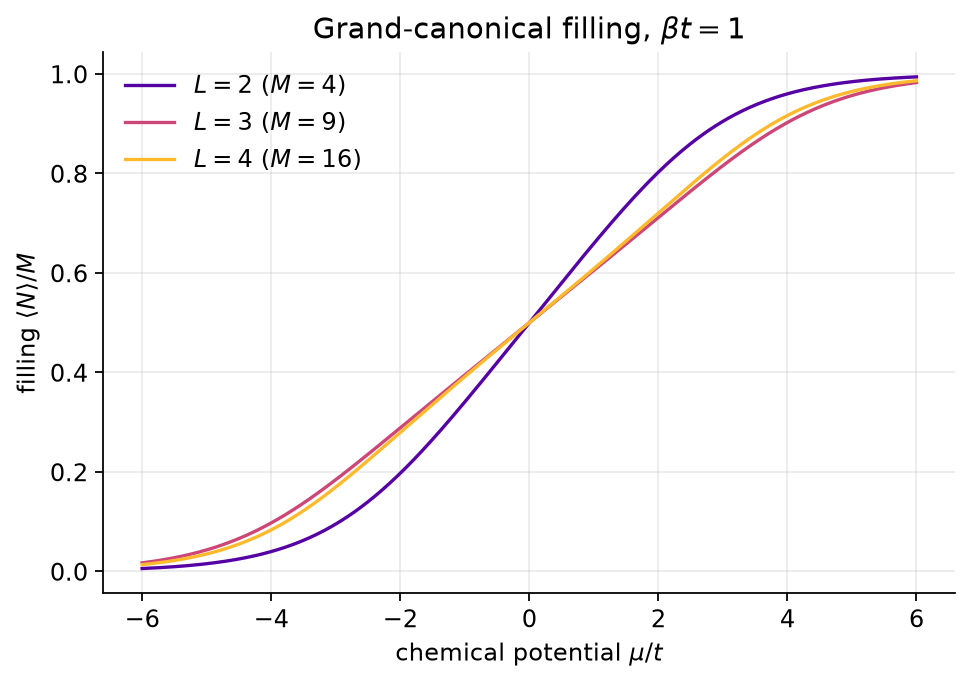
\includegraphics[width=\columnwidth]{fig3_mu_staircase.png}
\caption{Grand-canonical filling versus $\mu/t$ at $\beta t=1$,
$L=2,3,4$.}\label{fig:fill}
\end{figure}
\begin{figure}[t]\centering
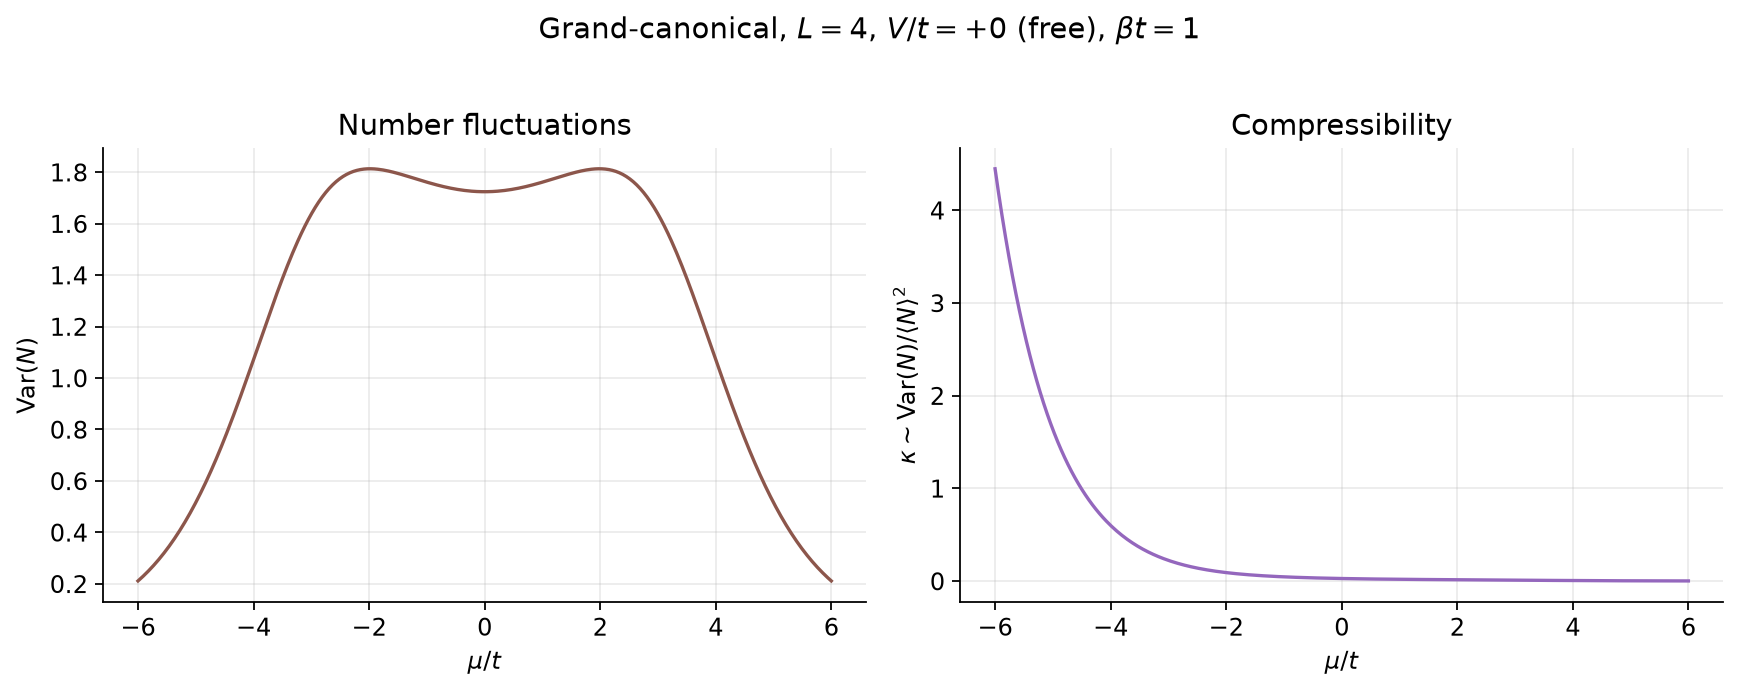
\includegraphics[width=\columnwidth]{fig4_number_fluctuations.png}
\caption{Number fluctuations and compressibility versus $\mu/t$ ($L=4$, $V=0$,
$\beta t=1$).}\label{fig:varn}
\end{figure}

\subsection{Ensemble energy comparison}
Figure~\ref{fig:eens} overlays canonical and grand-canonical energy per site at
matched $\mu^{*}$ (so $\avg{N}=N$). They coincide as $T\to0$ and open a small gap
at intermediate $T$---the finite-size inequivalence.
\begin{figure}[t]\centering
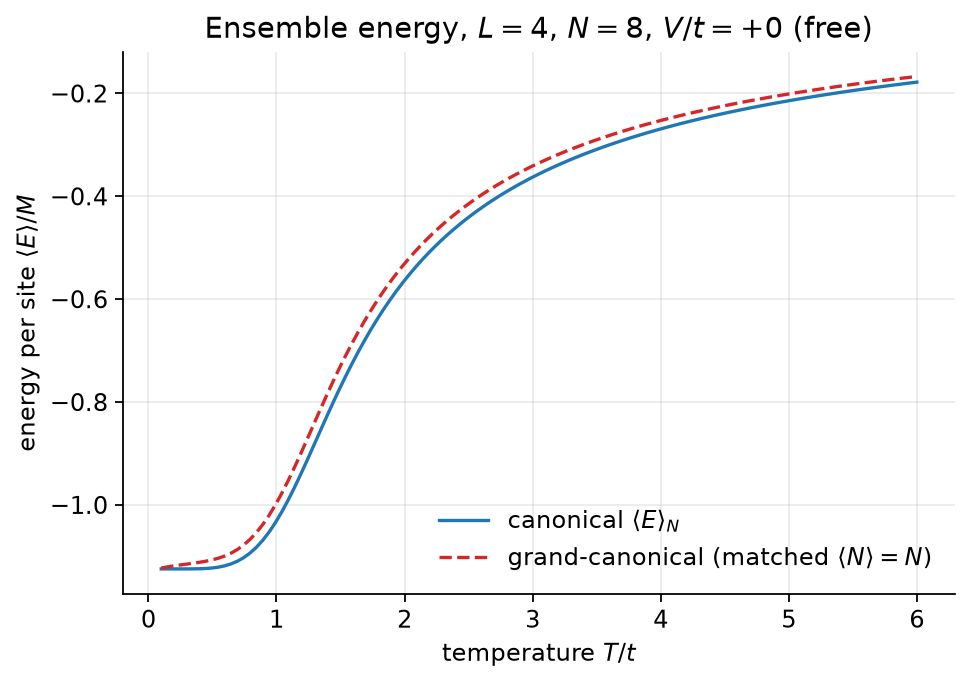
\includegraphics[width=\columnwidth]{fig5_energy_ensembles.png}
\caption{Canonical versus grand-canonical energy per site at matched particle
number ($L=4$, $N=8$, $V=0$).}\label{fig:eens}
\end{figure}

\subsection{Entropy and the caloric curve}
The canonical entropy per site $S/M=\beta\avg{E}/M+\ln Z_N/M$
(Fig.~\ref{fig:entropy}) rises from zero at $T\to0$ (a non-degenerate ground
state; the third law) and saturates at the infinite-temperature ceiling
$\ln(\dim)/M$. Attraction raises the entropy fastest and repulsion slowest,
mirroring the heat-capacity peak positions. Figure~\ref{fig:caloric} makes the
central methodological point graphically: the canonical caloric curve $T(E)$ is
smooth and monotone on the lower half of the spectrum, whereas the
microcanonical finite-difference temperature $1/(\partial S/\partial E)$
scatters around it and, crucially, turns \emph{negative} above the band center
($E\gtrsim0$)---the bounded spectrum's density-of-states maximum, where
$\partial S/\partial E$ changes sign. This is precisely the regime in which a
single-energy microcanonical thermometer fails, and it justifies anchoring the
equivalence analysis on fluctuation metrics rather than on $\partial
S/\partial E$.
\begin{figure}[t]\centering
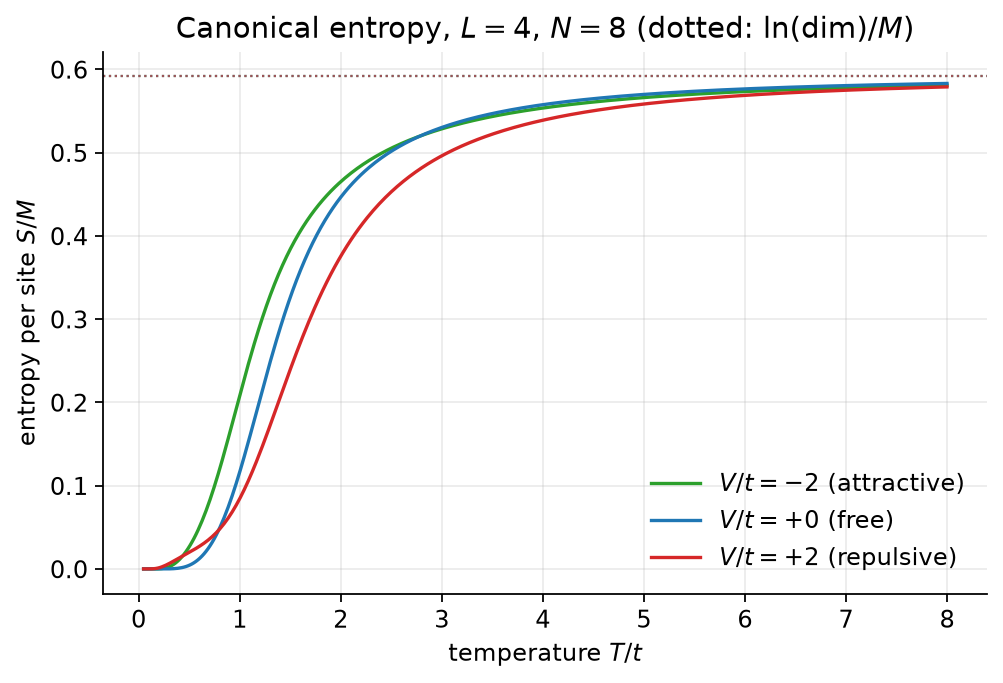
\includegraphics[width=\columnwidth]{fig8_entropy_temperature.png}
\caption{Canonical entropy per site $S/M$ versus temperature ($L=4$, $N=8$);
dotted lines mark the $T\to\infty$ ceiling $\ln(\dim)/M$.}\label{fig:entropy}
\end{figure}
\begin{figure}[t]\centering
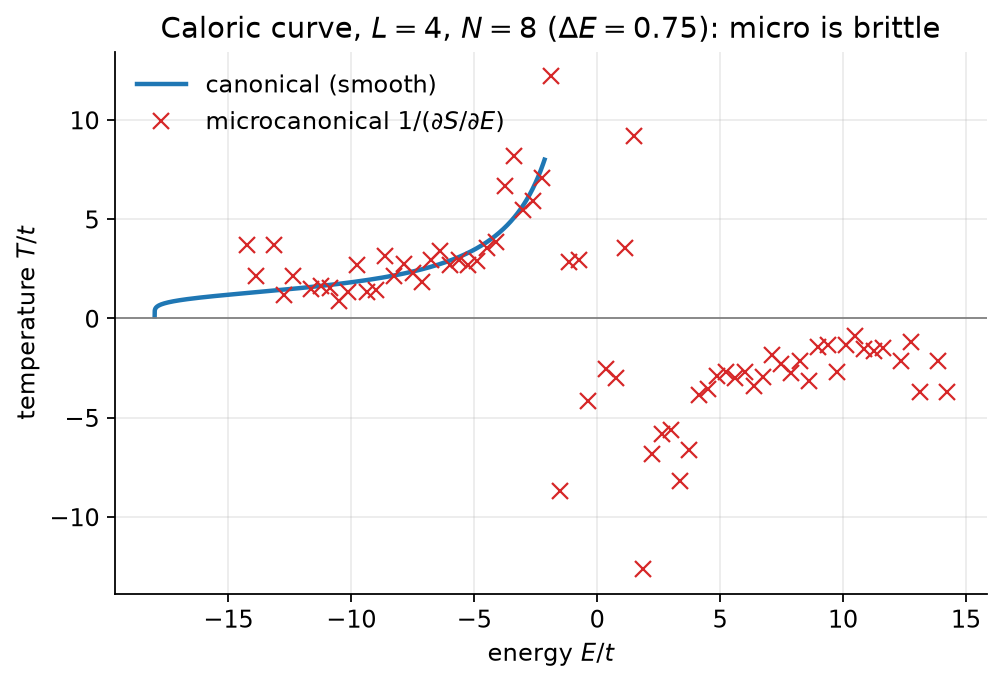
\includegraphics[width=\columnwidth]{fig11_caloric_curve.png}
\caption{Caloric curve $T(E)$: smooth canonical (line) versus microcanonical
finite differences (crosses) for $L=4$, $N=8$, $\Delta E=0.75$. The
microcanonical estimate is noisy and turns negative past the band center.}
\label{fig:caloric}
\end{figure}

\subsection{Finite-size scaling (central result)}
Figure~\ref{fig:scaling} and Table~\ref{tab:fits} present the three equivalence
metrics versus $M=L^2$ with power-law fits. Two conclusions stand out.
\emph{(i) Equivalence emerges for free and repulsive gases}: all metrics
decrease with size; the free-gas $r_N$ and $\Delta_E/M$ follow clean power laws
($R^2=1.00$) with exponents between $-0.6$ and $-0.9$, bracketing the
saddle-point expectation $M^{-1/2}$. \emph{(ii) Equivalence fails for the
attractive gas in the number channel}: $r_N$ stays large ($0.55$--$0.68$) and
flat with size ($p=-0.12$, $R^2=0.54$). This is the fingerprint of
canonical--grand inequivalence driven by the attractive gas's
clustering/phase-separation tendency: the grand ensemble supports large number
fluctuations between competing fillings that the fixed-$N$ canonical ensemble
forbids. The attractive \emph{energy} metrics still shrink---the inequivalence is
specific to the particle-number channel, where the instability lives.
\begin{figure*}[t]\centering
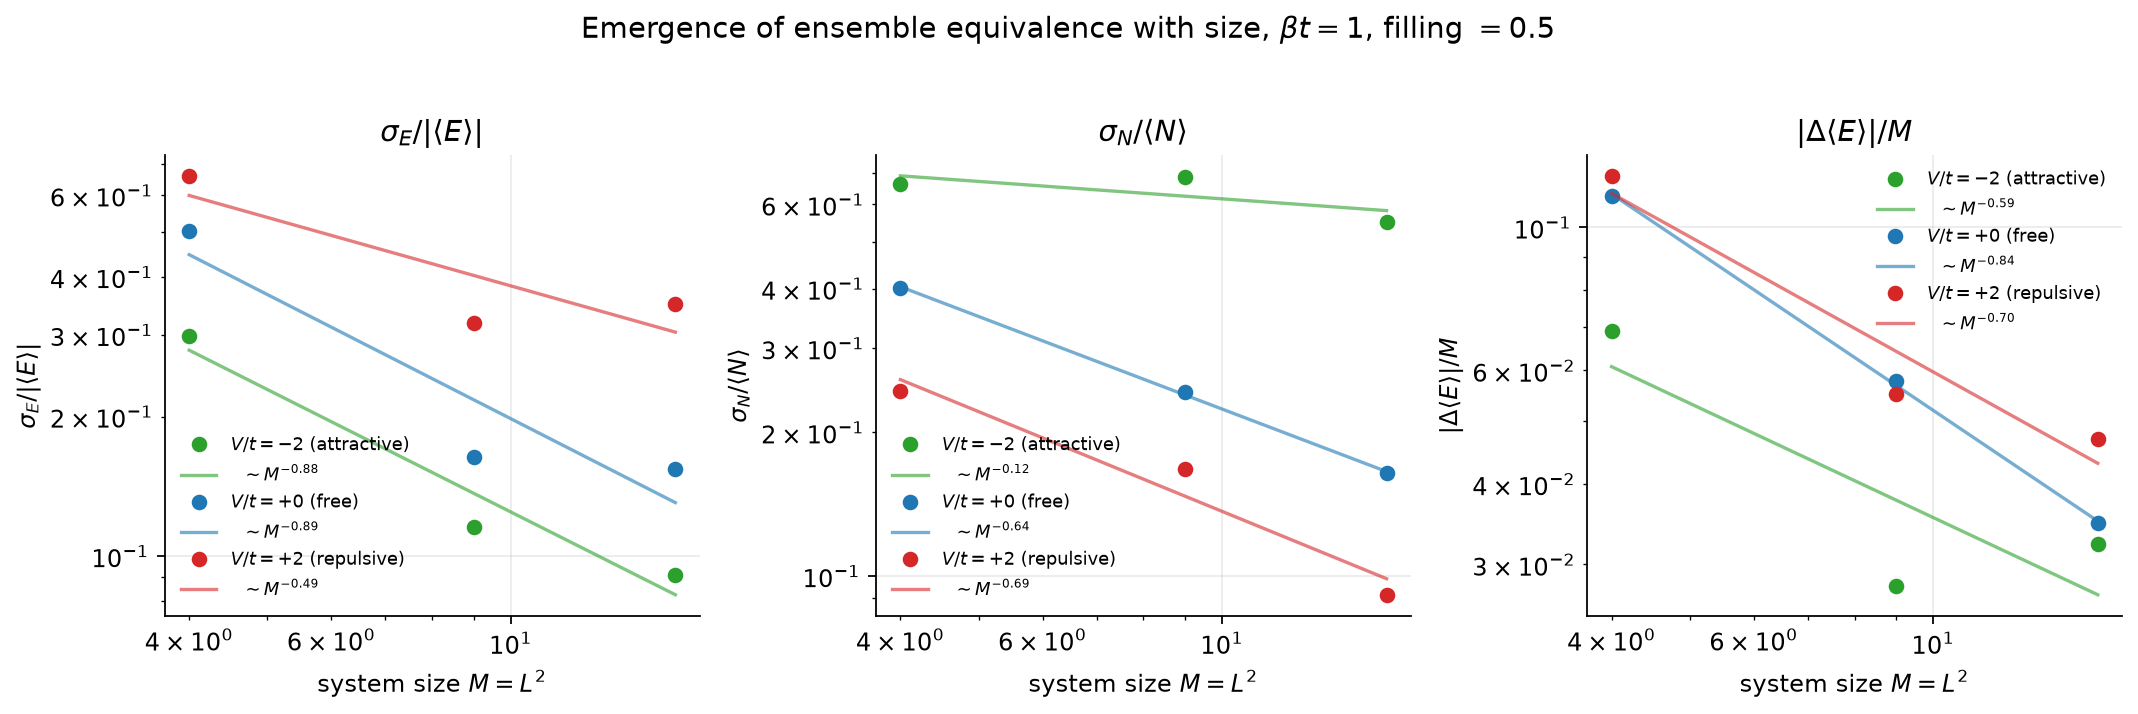
\includegraphics[width=0.92\textwidth]{fig6_scaling.png}
\caption{Finite-size scaling of $r_E$, $r_N$, and $\Delta_E/M$ for
$V/t=0,+2,-2$ at $\beta t=1$, half filling. Lines are power-law
fits.}\label{fig:scaling}
\end{figure*}

\begin{table}[t]\centering\small
\caption{Power-law exponent $p$ (fit $\propto M^{p}$), $R^2$, and measured values
at $M=4,9,16$. $\beta t=1$, half filling, periodic.}\label{tab:fits}
\begin{tabular}{rlrrrrr}
\toprule
$V/t$ & metric & $M{=}4$ & $M{=}9$ & $M{=}16$ & $p$ & $R^2$\\
\midrule
$0$  & $r_E$        & 0.503 & 0.164 & 0.154 & $-0.89$ & 0.86\\
$0$  & $r_N$        & 0.401 & 0.243 & 0.164 & $-0.64$ & 1.00\\
$0$  & $\Delta_E/M$ & 0.112 & 0.058 & 0.035 & $-0.84$ & 1.00\\
$+2$ & $r_E$        & 0.661 & 0.319 & 0.349 & $-0.49$ & 0.74\\
$+2$ & $r_N$        & 0.244 & 0.168 & 0.091 & $-0.69$ & 0.95\\
$+2$ & $\Delta_E/M$ & 0.120 & 0.055 & 0.047 & $-0.70$ & 0.93\\
$-2$ & $r_E$        & 0.298 & 0.116 & 0.091 & $-0.88$ & 0.95\\
$-2$ & $r_N$        & 0.664 & 0.684 & 0.553 & $-0.12$ & 0.54\\
$-2$ & $\Delta_E/M$ & 0.069 & 0.028 & 0.032 & $-0.59$ & 0.70\\
\bottomrule
\end{tabular}
\end{table}

\subsection{Interaction dependence}
Figure~\ref{fig:vdep} collects the metrics at $L=4$ versus $V/t$ over the three
cached couplings. A denser sweep is cheap at fixed $L=3$: Fig.~\ref{fig:vsweep}
resolves the full trend over $33$ values of $V/t$. The relative number
fluctuation $\sigma_N/\avg{N}$ rises smoothly and monotonically toward unity as
the interaction becomes more attractive---the continuous form of the
canonical--grand breakdown driven by clustering---while the relative energy
fluctuation grows instead with repulsion. The per-site energy gap stays small
and develops shallow minima. The anomaly is thus specific to the number channel
and to attraction, confirming it as a genuine physical effect rather than a
fitting artifact.
\begin{figure}[t]\centering
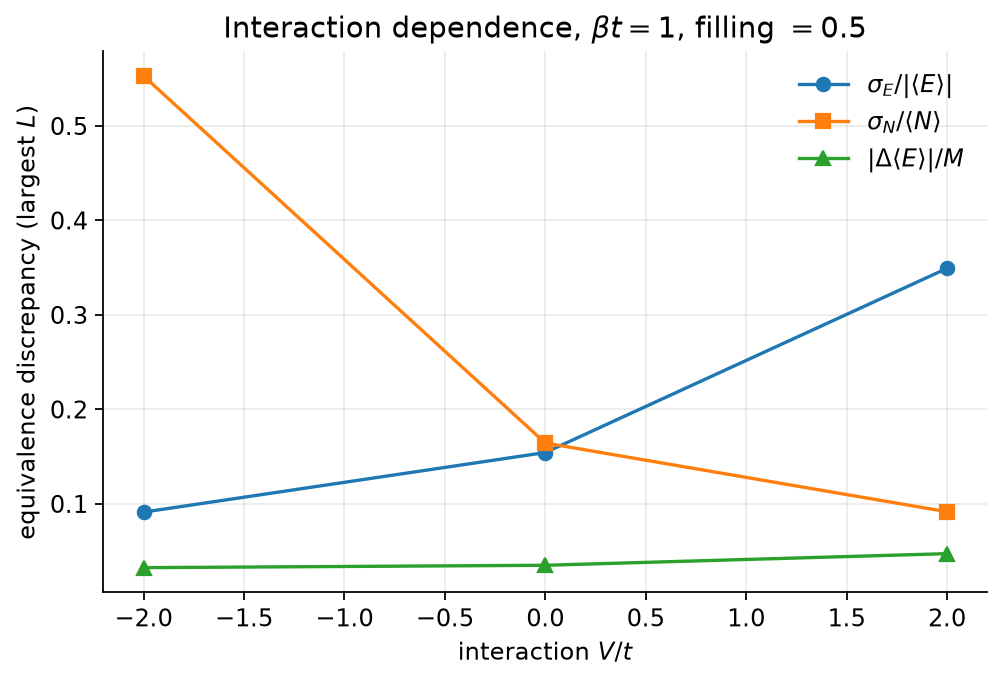
\includegraphics[width=\columnwidth]{fig7_interaction.png}
\caption{Equivalence metrics at $L=4$ versus $V/t$ (three cached
couplings).}\label{fig:vdep}
\end{figure}
\begin{figure}[t]\centering
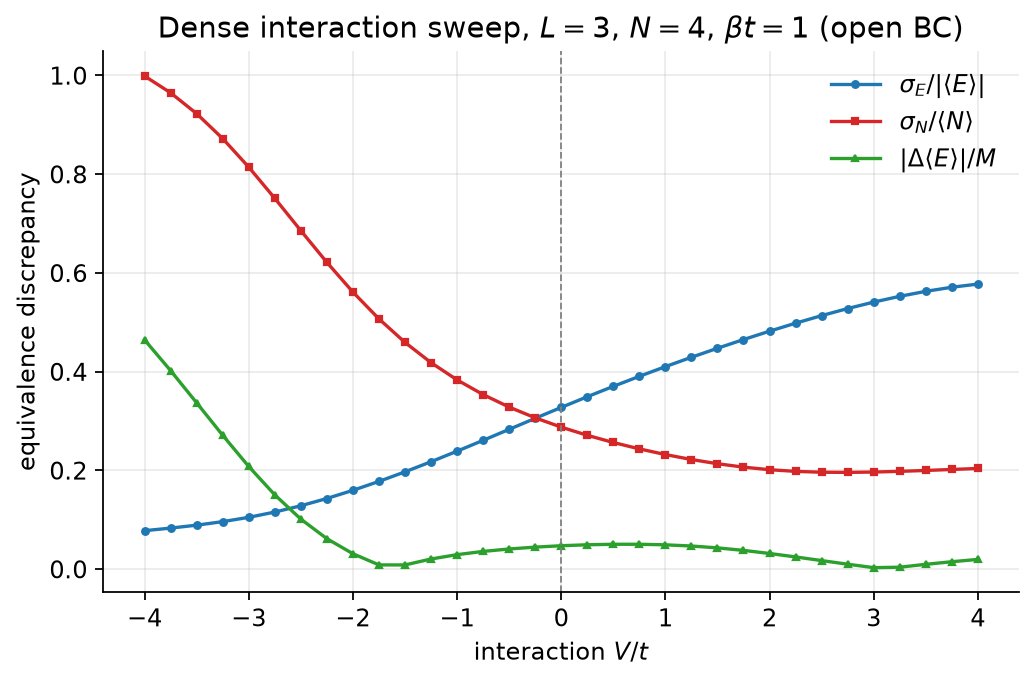
\includegraphics[width=\columnwidth]{fig12_interaction_sweep.png}
\caption{Dense interaction sweep at fixed $L=3$ ($33$ couplings, open BC,
$\beta t=1$): $\sigma_N/\avg{N}$ grows toward unity with attraction, the
number-channel signature of ensemble inequivalence.}\label{fig:vsweep}
\end{figure}

\section{Discussion}
\textbf{Why fluctuations, not thermometry.} The canonical distribution is the
Laplace transform of the microcanonical density of states, and equivalence is the
statement that this transform is saddle-point dominated. The width
$\sigma_E/|\avg{E}|$ measures saddle sharpness directly; it is a smooth spectral
sum, free of the differentiation noise that cripples $\partial S/\partial E$ on a
discrete spectrum. The same holds for $\sigma_N/\avg{N}$. The fluctuation metrics
are thus both robust and correct.

\textbf{The attractive anomaly.} An attractive nearest-neighbor interaction
lowers the energy of clustered configurations, driving a low-temperature
tendency toward phase separation. In the grand ensemble this yields a broad
$P(N)$ with large $\mathrm{Var}(N)$ that does not self-average at these sizes;
the canonical ensemble, with $N$ pinned, cannot access the competing fillings, so
the ensembles disagree. This is the finite-size precursor of the thermodynamic
failure of equivalence at first-order transitions.

\textbf{Limitations.} With only $M=4,9,16$, the exponents are indicative, not
precise, and the $M=4$ point leverages the fits---doubly so because the $L=2$
periodic lattice de-duplicates to a single-bonded four-site ring rather than the
true double-bonded two-torus (its $N=1$ band is $\{-2t,0,0,2t\}$ instead of the
dispersion minimum $-4t$), so it is a slightly different lattice from the $L=3,4$
members of the sequence. The $L=3,4$ single-particle spectra reproduce the exact
tight-binding band $-2t[\cos k_x+\cos k_y]$ to machine precision. Results are at a
single temperature $\beta t=1$; the microcanonical $T,\mu$ are reported only as a
window-sensitive diagnostic; the bounded spectrum admits negative-temperature
states that the fluctuation metrics sidestep. The dense interaction sweep of
Fig.~\ref{fig:vsweep} is computed at fixed $L=3$ (open boundaries), where many
$V/t$ values are inexpensive.

\section{Conclusion}
Using numerically exact diagonalization of the 2D hard-core Bose--Hubbard model,
we gave a transparent, reproducible account of how ensemble equivalence emerges
with system size in an interacting quantum lattice gas. By recognizing the
ill-conditioning of finite-difference microcanonical thermometry and instead
measuring equivalence through robust fluctuation observables, we demonstrated
monotone power-law convergence for the free and repulsive gases and a clear
breakdown of canonical--grand equivalence in the number channel for the
attractive gas---the finite-size signature of its phase-separation instability.

\paragraph{Author contributions.} P.\ Das, A.\ Shakya, and D.\ Thakur conceived
the study, developed the exact-diagonalization and ensemble framework, performed
the calculations and analysis, and wrote the manuscript.

\begin{thebibliography}{9}
\small
\bibitem{greiner} M.~Greiner \emph{et al.}, Nature \textbf{415}, 39 (2002).
\bibitem{bloch} I.~Bloch, J.~Dalibard, W.~Zwerger, Rev.\ Mod.\ Phys.\ \textbf{80}, 885 (2008).
\bibitem{touchette} H.~Touchette, Phys.\ Rep.\ \textbf{478}, 1 (2009).
\bibitem{pathria} R.~K.~Pathria, P.~D.~Beale, \emph{Statistical Mechanics}, 3rd ed.\ (Elsevier, 2011).
\bibitem{sandvik} A.~W.~Sandvik, AIP Conf.\ Proc.\ \textbf{1297}, 135 (2010).
\bibitem{dauxois} T.~Dauxois \emph{et al.}\ (eds.), \emph{Dynamics and Thermodynamics of Systems with Long-Range Interactions} (Springer, 2002).
\end{thebibliography}

\end{document}
